\documentclass[a4paper]{article}

\usepackage[english]{babel}
\usepackage[utf8]{inputenc}
\usepackage{amsmath}
\usepackage{graphicx}
\usepackage[colorinlistoftodos]{todonotes}

\title{C\&W On Multiple Phenotype GWA Studies}

\author{Omid Shams Solari}

\date{\today}

\begin{document}
\maketitle

\begin{abstract}
The case under study in this paper is a GWA study of genes under selection for multiple phenotypes under exposure to predation of Daphnia Magna. LASSO regularization and Ridge regression are used for prediction. Then considering the multiple correlated phenotypes, Curds \& Whey method is used along with RR and LASSO to increase the prediction accuracy under the quadratic loss.
\end{abstract}

\section{Introduction}
\label{sec:introduction}

Genome Wide Association Studies, GWAS, is referred to a group of widely popular studies with the aim of finding associations between genetic variants and traits. Genetic variants are usually single-nucleotide polymorphisms, i.e. SNPs, or linkage disequilibruims and traits can vary from phenotypes like height and weight to susceptibility to different diseases.\\
The focus of this project is to find different associations between genetic variants and various physical traits in 19 populations of Daphnia Magna each from a different location. 188 individuals were sequenced which provide the full genome sequence for each of the populations, of which phenotypic traits of 123 individuals were available. 12 traits were recorded for each of the individuals. The associated genetic variants will point to the genes and mechanisms under selection for ecological variants which is \textit{Fish Predation} here.\\
Few differences sets this study apart from any other GWA study in other organisms. The first difference is that because of short generation time of Daphnia Magna, genetic variants are more likely to be found given a limited time comparing to other organisms with much longer generation time. Daphnia is very adaptable to different ecosystems so their sustainable colonies can be found in many different locations which makes it a very good organism for studying spatial variations. They are equipped with an amazing behavior which make them very suitable for genomics and that is the capability to have both sexual and clonal reproduction. Having a clonally reproduced population means that they have identical DNAs which provides immense predictive power comparing to organisms where the DNAs are different. Yet another exciting behavior of Daphnia is that their fertile eggs can go into diapause and stay in the sediments for centuries and then be hatched. This makes them ideal for studies of temporal variations. \\


\section{EDA}
\label{sec:data}
The dataset at hand is two parts: 
\begin{itemize}
\item The genotypic part of the dataset which contains the genotypic variants and are treated here as the predictors.
\item The phenotypic part which contains the traits of the organisms and are treated here as the response variables.
\end{itemize}
In this chapter we explore through the different parts of the data.

\subsection{Genotypic Data}
A total of 1018297 SNP calls from 188 individuals were obtained through \textit{The Daphnia Consortium}. As the first pass strict filters were imposed on the SNPs to both reduce the size of the dataset as much as possible and also see if it's possible to find the most important SNPs although may be too few. As the first filter only those sites were chosen that in which at least one individual contained a SNP which contained the alternative allele on both chromosomes, since we're dealing with a diploid organism. Then looking at the histogram of the Phred-scaled marginal probability of the called genotypes and the read depth as you see in Figure \ref{fig:hist}, only SNPs with a Phred score larger than 90 and read depth larger than 10 were chosen which left us with about 154000 SNPs.


\begin{figure}
\centering
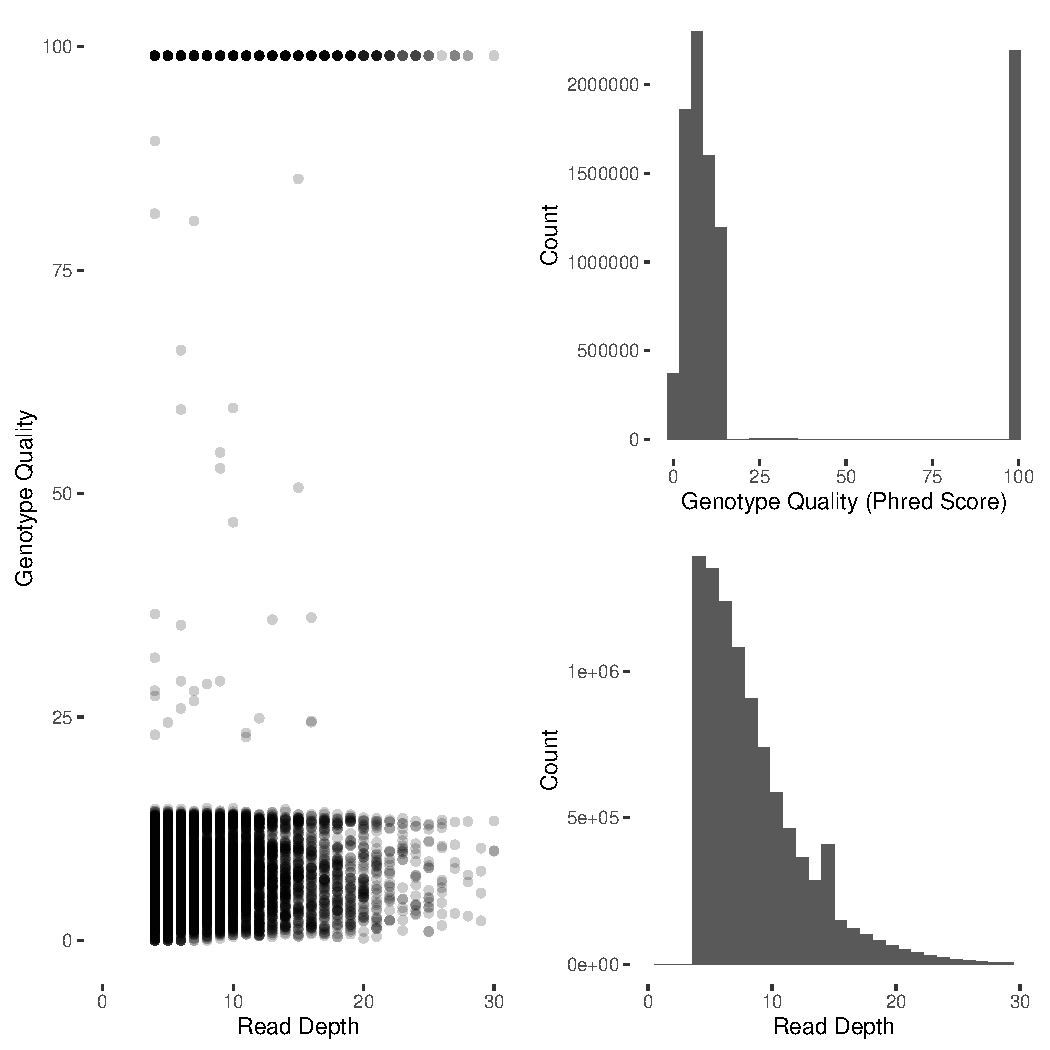
\includegraphics[width=0.8\textwidth]{hist.pdf}
\label{fig:hist}
\caption{Read depth and genotype quality distributions}
\end{figure}

\subsection{Phenotypic Data}

Due to an absence of unified naming protocol, the sample names in the phenotype dataset were different from their names in the genotypic variations dataset. Each sample was matched and double checked with the biologists in charge to make sure the phenotypes belong to the correct sample. \\
Since the different phenotypes had very different ranges and variations and since we were going to use the \textit{Generalized Cross-Validation-based Curds\&Whey} which requires the resonses to be normally distributed, the dataset was centered, scaled and transformed using the Cox-Box transformation. All the analysis is done on this transformed matrix.\\
First to take a look at how coherent the data set is and to find the outlier samples, we plotted the first two principle components of the phenotypes, although 8 principle components were needed to capture 95\% of the variance. Figure \ref{fig:pca} shows the first two PCs plotted against each other with the 7 outliers labeled.

\begin{figure}
\centering
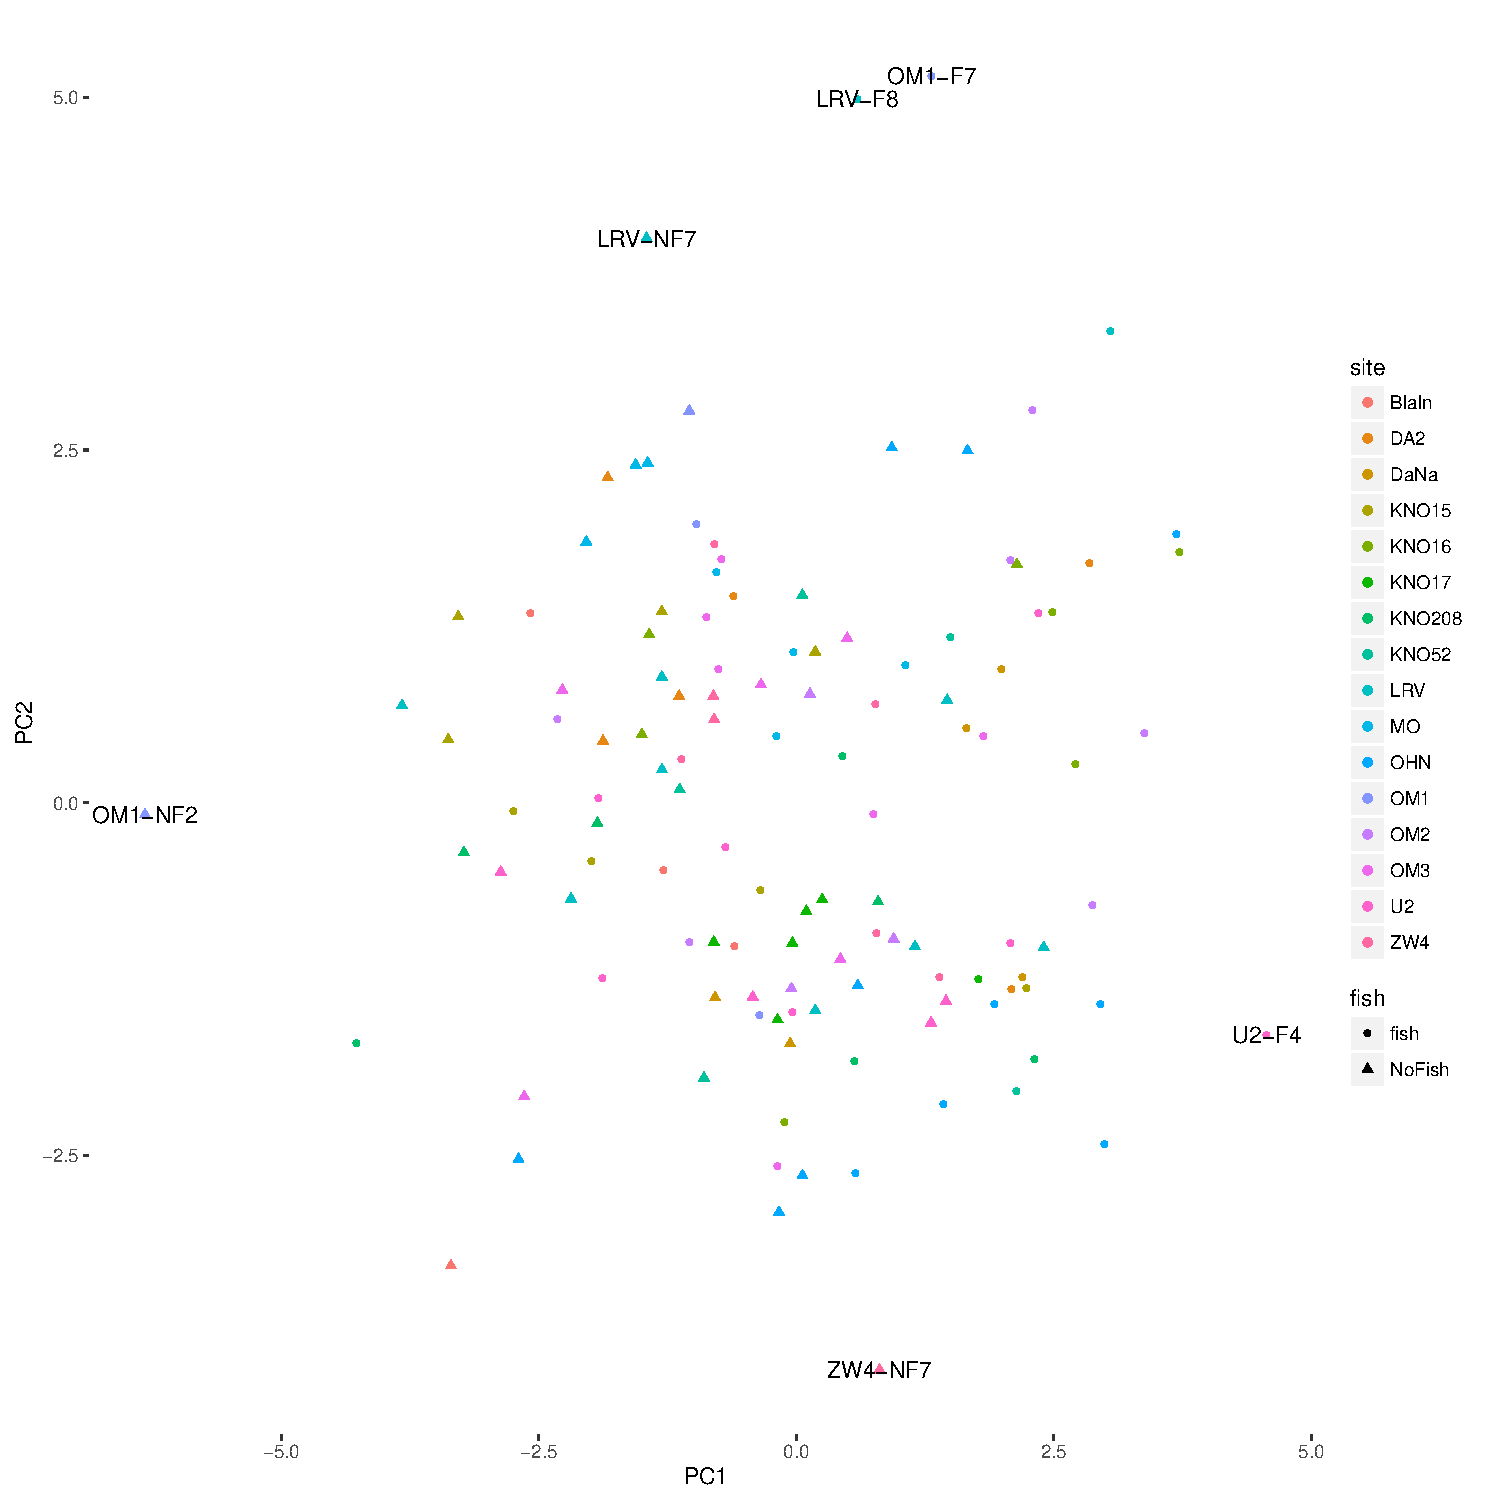
\includegraphics[width = .9\textwidth]{pca.pdf}
\label{fig:pca}
\caption{The first two PCs of the transformed dataset.}
\end{figure}


In Figure \ref{fig:corrplot} the correlation matrix of all the phenotypes is shown. There are highly correlated and anti-correlated phenotypes in this dataset. For example \textit{Age of mother in the second clutch, age of mother at maturity} and \textit{age of mother in the first clutch} are a group of highly correlated phenotypes. We hope to be able to use this structure between phenotypes to improve the prediction accuracy.\\


\begin{figure}

\centering
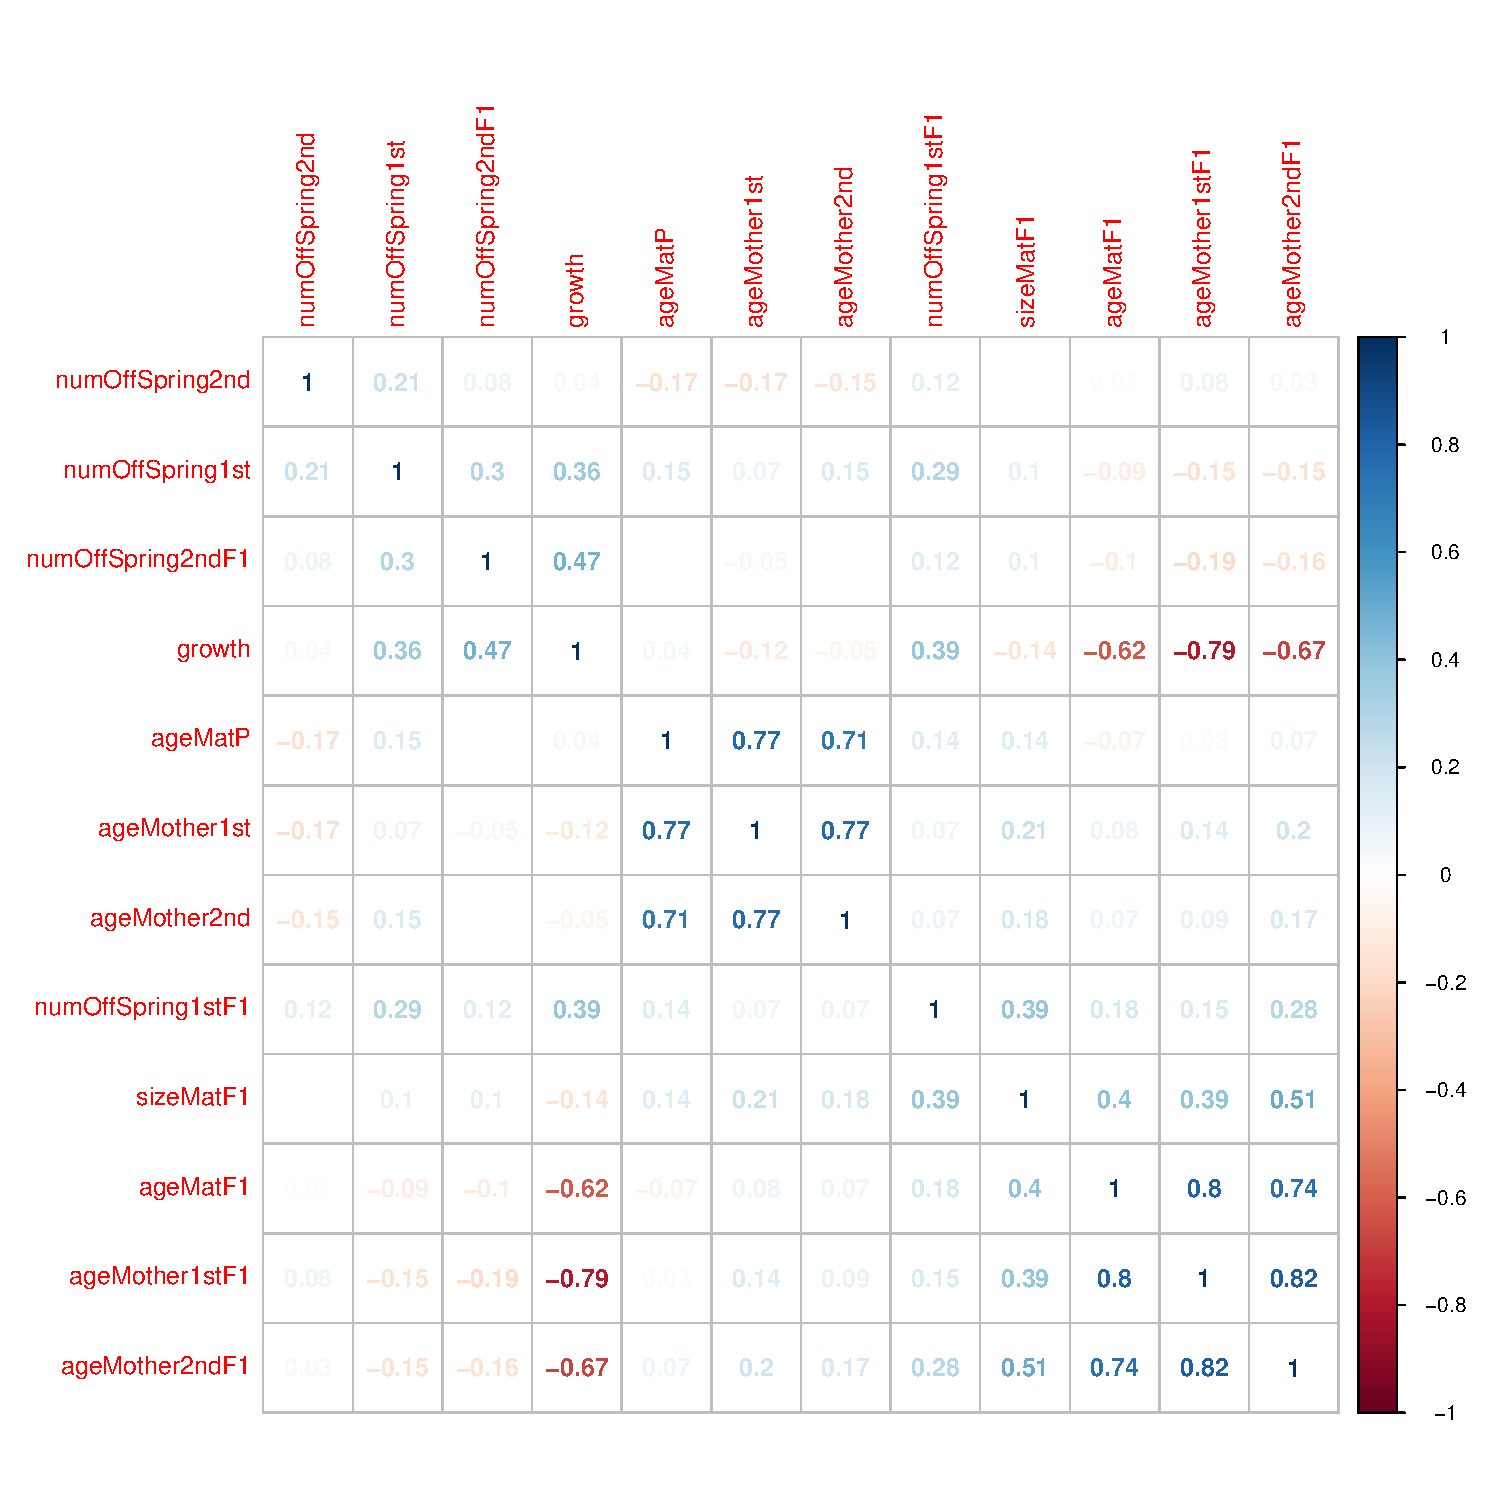
\includegraphics[width=1\textwidth]{corrplotPhenotype.pdf}
\label{fig:corrplot}
\caption{Corrplot of all phenotypes, Pearson correlation is computed}
\end{figure}

If we are going to find the genes under selection for predation, the difference in the measured phenotypes for the two conditions of predation/no-predation should be meaningful. Figure \ref{fig:boxplot} compares the distributions of different phenotypes between the control and treatment, i.e. predation or no-predation. In table \ref{tb:pval} the results of two-tailed two-sample test of significance of means is done on each phenotype. Using a threshold of 0.05 for the significance, 5 of the 12 phenotypes do not differ significantly between the control and the treatment. These phenotypes were filtered.

\begin{figure}
\centering
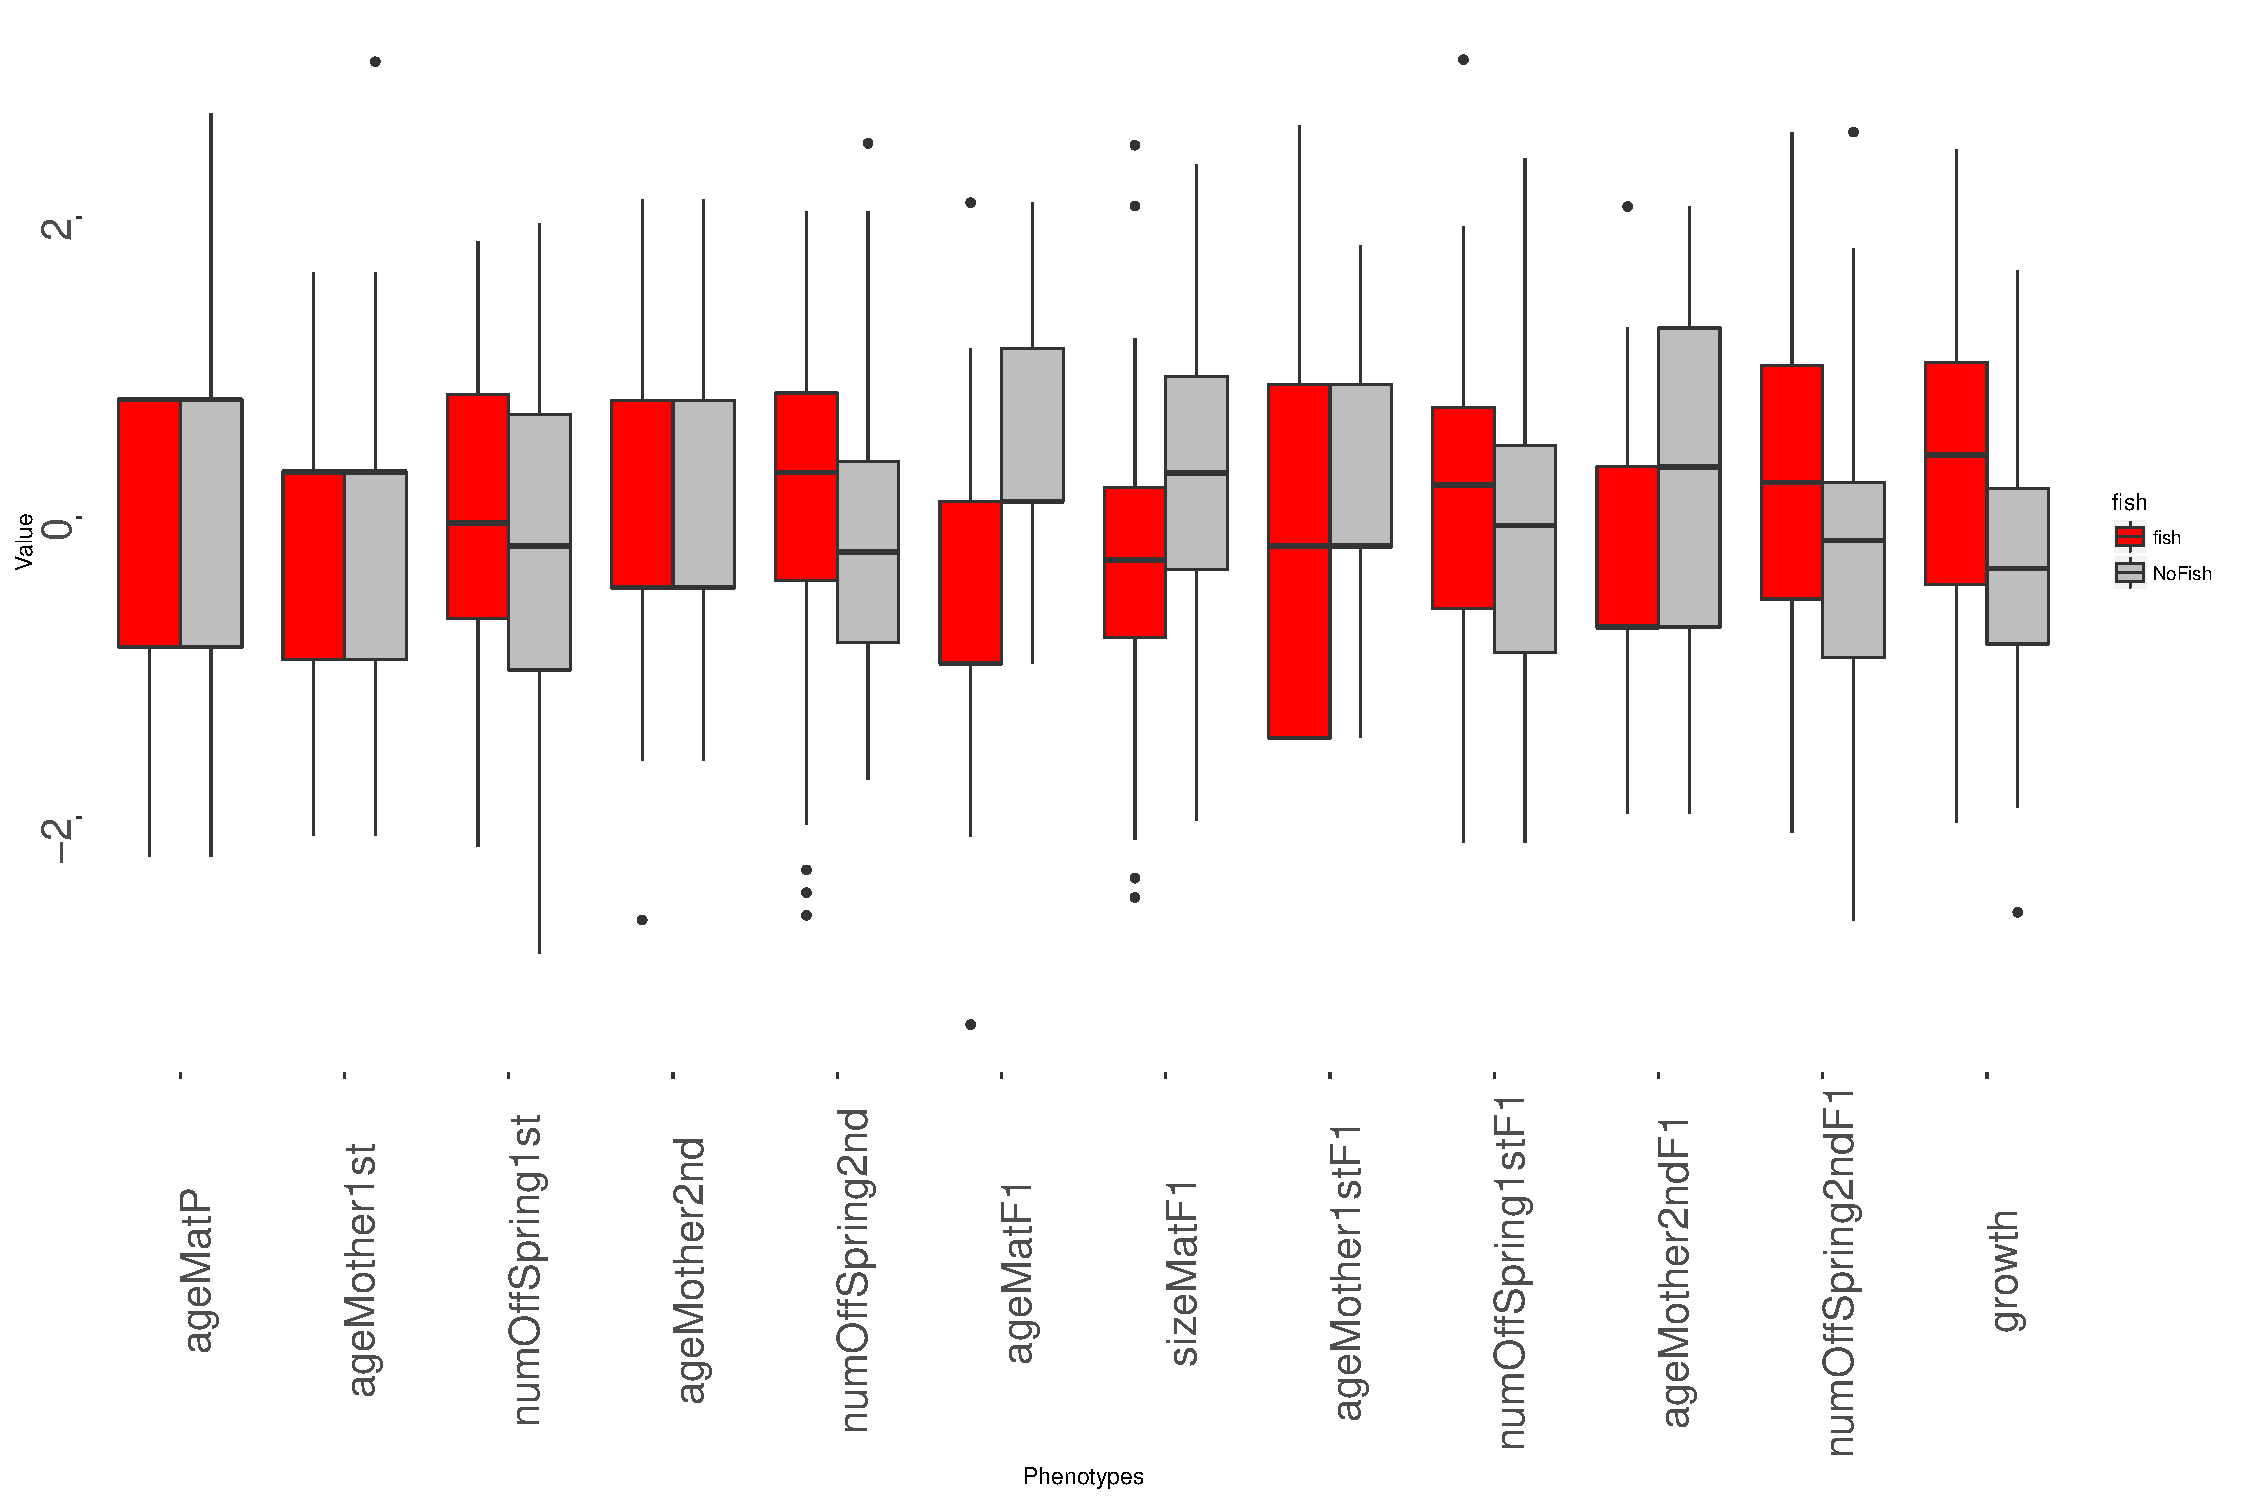
\includegraphics[width = .9\textwidth]{boxplot.pdf}
\label{fig:boxplot}
\caption{Phenotype distribution.}
\end{figure}

\begin{table}
\caption{Two-tailed two-sample test of significance of the difference in means}
\label{tb:pval}
\begin{center}
\begin{tabular}{ |l|l|l| }
  \hline
  Phenotype & t-Statistic & P-value \\
  \hline
  ageMatP  &         -0.2384 &0.8119\\
ageMother1st    &  -1.6165 &0.1089\\
numOffSpring1st   & 0.8418 &0.4016\\
ageMother2nd     & -1.9701& 0.0512\\
numOffSpring2nd   & 1.4582& 0.1475\\
ageMatF1         & -2.9446& 0.0039\\
sizeMatF1       &  -3.4709& 0.0007\\
ageMother1stF1   & -2.9482& 0.0038\\
numOffSpring1stF1 & 0.9070& 0.3662\\
ageMother2ndF1   & -3.6670& 0.0003\\
numOffSpring2ndF1 & 2.1287& 0.0354\\
growth            & 4.0152& 0.0001\\
  \hline
\end{tabular}
\end{center}
\end{table}



\section{Theory}

As mentioned in the introduction, we want to access that under quadratic loss, how much better we are off if we consider all response variables, here phenotypes? Can we use the correlation structure between them to improve our prediction accuracy?\\
Curds\&Whey which is proposed by Breiman and Friedman\cite{breiman} suggests a transformation which includes a rotation along the canonical coordinates of response variables, a shrinkage which shrinks each response variable separately and then another rotation back from the canonical coordinates to the original coordinates.\\
Breiman and Friedman(1997)\cite{breiman} present three variations of Curds\&Whey Method:
\begin{enumerate}
\item Canonical Co-ordinate Shrinkage
\item Generalized Cross-Validation Curds\&Whey
\item Fully Cross-Validated Curds\&Whey
\end{enumerate}

All of which result in an "optimal" matrix $B_{q \times q}$, where shrinkage by which results in improved prediction accuracy in $l_2-norm$ sense,

\begin{equation}
\begin{split}
\tilde{y} &= \mathbf{B}\hat{y}\\
E[y - \tilde{y}]^2 &< E[y - \hat{y}]^2
\end{split}
\end{equation}

Since the \textit{Canonical Co-ordinate Shrinkage} relies on the assumption that the predictors and the errors are independent, only the cross-validation-based Curds\&Whey methods are implemented and compared. Also since in this project $p>>N$, the system is undetermined. So we use Ridge-Regression along with C\&W. Ultimately three methods are implemented and compared: RR, i.e. separate Ridge Regression, C\&W-RR-GCV, i.e. Curds\&Whey Ridge Regression using Generalized Cross-Validation and C\&W-RR-FCV, i.e. Curds\&Whey Ridge Regression Fully-Cross-Validated.

\subsection{Separate Ridge Regression}
In this approach an RR model is fit to each response variable separately, yielding the coefficient matrix $\hat{\mathbf{A}}_{\lambda} \in \mathcal{R}^{q \times p}$.

\begin{equation}
\hat{\mathbf{A}}_{\lambda} = (\mathbf{X}^T\mathbf{X} + \lambda \mathbf{I}_p)^{-1} \mathbf{X}^T\mathbf{Y}
\end{equation}

Where the Ridge coefficients are the solution to the penalized least squares.

\begin{equation}
\{ \hat{a}_{ij} \}_{j = 1}^p = argmin_{\{ a_j \}_1^p} \{ \sum_{n = 1}^N (y_{ni} - \sum_{j = 1}^p a_jx_{nj})^2 \} + \lambda_i \sum_{j = 1}^p a_j^2
\end{equation}

Which in turn is used to attain the fitted values,
\begin{equation}
\mathbf{\hat{y}}(\lambda) = \hat{\mathbf{A}}_{\lambda} \mathbf{x}
\end{equation}

Where full cross-validation was used to choose the optimal $\lambda$.

\begin{equation}
\hat{\lambda} = argmin_{\lambda}[\sum_{i = 1}^{q}\sum_{n = 1}^N \{ y_{ni} - \hat{y}_{\setminus ni}(\lambda)  \}^2]
\end{equation}

\subsection{Cross-Validation-Based Methods}
Obviously the optimal shrinkage is obtained by regressing the responses in the test set on their estimates attained by fitting our model. One can come closer to this ideal by the use of cross-validation, where each or a group of observations are separated and used as future observations. Putting this idea mathematically,

\begin{equation}
\{ b_{ik} \}_{k = 1}^q = argmin_{\{ \beta_k \}_1^q} \{ \sum_{n = 1}^N (y_{ni} - \sum_{k = 1}^q \beta_k \hat{y}_{\setminus nk})^2 \}
\end{equation}

Where $\hat{y}_{\setminus nk}$ is the OLS fitted value of the kth response of the nth observation, obtained by removing it from the training set, i.e. treating it as if it belongs to the test set. Needless to say that one may use k-fold cross-validation instead of this fully-cross-validated measure.

In practice, having $\hat{\lambda}$, the C\&W-RR estimates are computed by,

\begin{equation}
\tilde{\mathbf{y}} = \mathbf{B}\hat{y} = (\mathbf{\hat{T}}^{-1}\mathbf{D}\mathbf{\hat{T}})\mathbf{\hat{A}}_{\hat{\lambda}}\mathbf{x}
\end{equation}
 Where $\mathbf{D}_{q \times q}$ is a diagonal matrix and $\mathbf{\hat{T}} \in \mathbf{R}^{q \times q}$ is obtained by a canonical correlation analysis between $\mathbf{Y}$ and $\mathbf{\hat{Y}}$,
 
 \begin{equation}
 \label{eq:qhat}
\mathbf{\hat{Q}} = \mathbf{Y}^T\hat{\mathbf{Y}}_{\hat{\lambda}}(\mathbf{Y}^T\mathbf{Y})^{-1}\hat{\mathbf{Y}}_{\hat{\lambda}}^T\mathbf{Y}(\hat{\mathbf{Y}}_{\hat{\lambda}}^T\hat{\mathbf{Y}}_{\hat{\lambda}})^{-1} = \hat{\mathbf{T}}^{-1}\hat{\mathbf{C}}^2\hat{\mathbf{T}}
\end{equation}

Where the RHS of Equation \ref{eq:qhat} is the eigen-decomposition of $\hat{\mathbf{Q}}$, so  $\hat{\mathbf{C}}^2_{q \times q}$ is a diagonal matrix. 

The main difference between the \textit{Generalized Cross-Validation} and \textit{Fully Cross-Validated} methods is in how the diagonal matrix $\mathbf{D}$ is found. 

\subsubsection{Generalized Cross-Validation Curds\&Whey}
As discussed in Breiman(1997)\cite{breiman}, one may use Equation \ref{eq:di} to estimated the diagonal matrix $\mathbf{D}$. 

\begin{equation}
\label{eq:di}
\hat{d}_i = \frac{(1- r)(\hat{c}_i^2 - r)}{(1 - r)^2\hat{c}_i^2 + r^2(1 - \hat{c}_i^2)} \qquad i = 1, ..., q
\end{equation}

We perform a positive part shrinkage, so

\begin{equation}
\hat{d}_i = max(\hat{d}_i, 0)
\end{equation}

As suggested in Breiman(1997)\cite{breiman}, $r$ is estimated by

\begin{equation}
\hat{r} = \frac{1}{N} trace\{ \mathbf{X}(\mathbf{X}^T \mathbf{X} + \hat{\lambda} \mathbf{I}_p)^{-1}  \mathbf{X}^T \}
\end{equation}

Since for all the cases $\hat{\lambda}$ was much smaller than the diagonal elements of $\mathbf{X^TX}$,
\begin{equation}
\label{eq:gcv}
\hat{r} = \frac{1}{N}trace\{ \mathbf{H} \} = \frac{p}{N}
\end{equation}

Where $\mathbf{H}$ is the familiar hat matrix. This procedure is  called C\&W-GCV or Generalized Cross-Validation-based Curds\&Whey.

\subsubsection{Fully Cross-Validated Curds\&Whey}
Since the estimations and assumptions in Equations \ref{eq:di} through \ref{eq:gcv} might be inaccurate, a fully cross-validated method also was implemented. In this approach each element of the diagonal matrix $\mathbf{D}$ is estimated using k-fold cross-validation.

\begin{equation}
\mathbf{D} = argmin_{\Delta = diag} [\sum_{i = 1}^q \sum_{n = 1}^N \{ y_{ni} - (\hat{T}_{\setminus n}^{-1} \Delta \hat{T}_{\setminus n} \hat{y}_{\setminus n})_i \}^2]
\end{equation}


In this approach the training set is divided into a new training set and test set and then an RR model is fit to the new training set and then it's used to predict the new test set values. Also using Equation \ref{eq:qhat}, $\hat{\mathbf{T}}$ is computed. Then both the true values and the fitted values of the new test set are transformed using $\hat{\mathbf{T}}$. Regressing the new test set values on its true values separately for each response variable,

\begin{equation}
\hat{\mathbf{T}}\tilde{y} = \mathbf{D} (\hat{\mathbf{T}} \hat{y}
\end{equation}

matrix $\mathbf{D}$ is estimated for each fold. The average value of the shrinkage values with the range $[0,1]$ imposed on them was chosen as the optimal shrinkage matrix.

\subsection{Hypothesis Testing}
To assess the significance of the difference between the three methods, RR , C\&W-RR-GCV and C\&W-RR-FCV, the algorithm is repeated K times on a randomly sampled training set and the prediction accuracy is computed using the MSE. Then a two-tailed t-test is performed to examine whether the difference between the means of the two samples with equal size but different variance is used.

\begin{equation}
t = \frac{\bar{X}_1 - \bar{X}_2}{{S}_{X_1X_2}\sqrt{\frac{1}{n}}} \qquad \#DoF = 2(n-1) 
\end{equation}

Where $$S_{X_1X_2} = \sqrt{S_{X_1}^2 + S_{X_2}^2}$$




\section{Analysis}
To make the computation manageable on a single laptop given the time constraint, only the top 10000 scoring Sites were chosen which contain 446211 high-score SNPs. Since $p >>N$, where p is the number of predictors and N is the number of samples, the system is under-determined. To remedy this as we discussed in the previous section, Ridge Regression along with C\&W was used using both \textit{Generalized Cross-Validation} and \textit{Fully Cross-Validated} methods as discussed in detail in the previous section.\\
First, the dataset was divided into a training set which contained 100 samples and the remaining 32 samples were assigned to the test set. In each run an RR model was fit to each response variable and the optimum constraint parameter was found by full cross-validation. Then the shrinkage matrix was found using both methods and then used to shrink the predicted value of RR for the test set. This process was repeated 50 times and for each phenotype the \textit{Total Squared Error} was computed. All three methods are compared in Figure \ref{fig:boxplotMethods}.

\begin{figure}
\centering
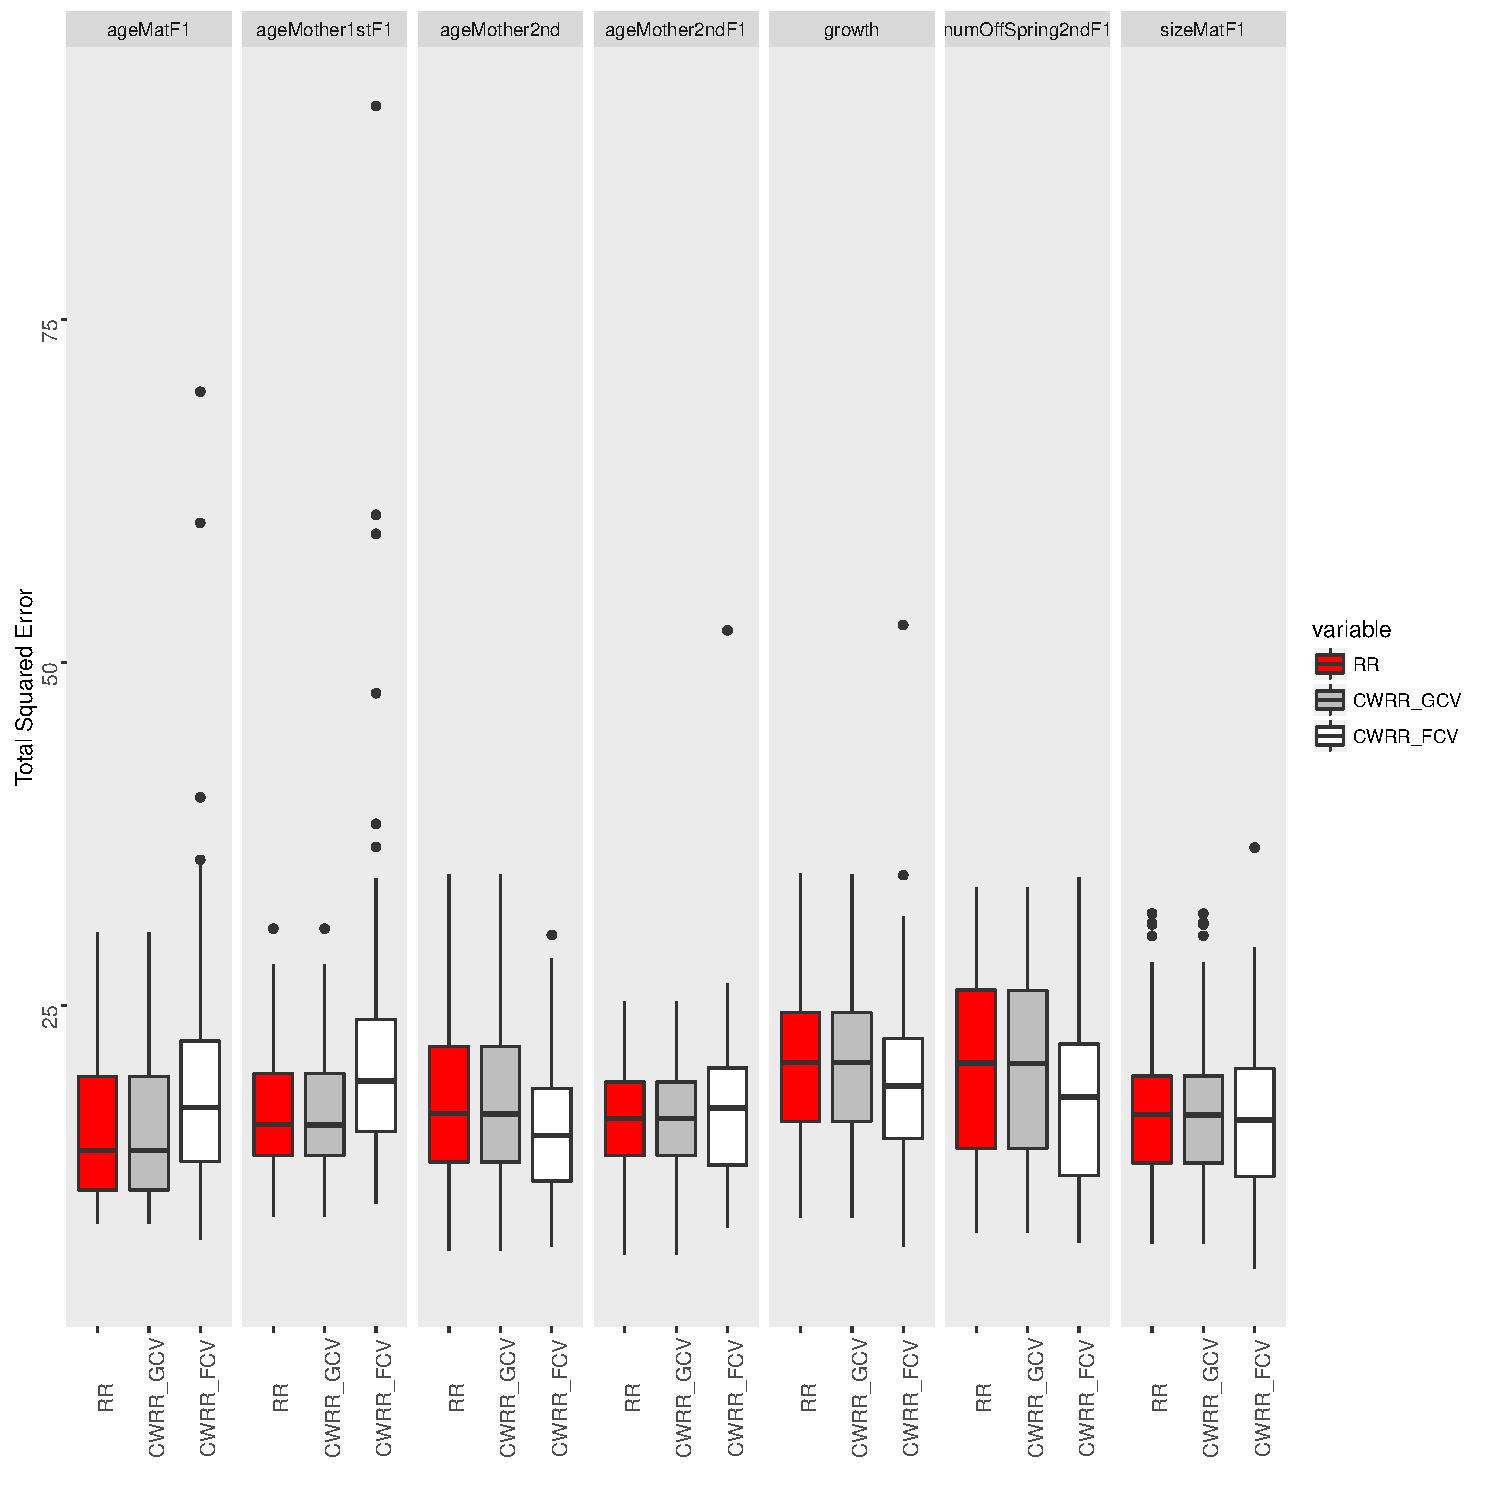
\includegraphics[width = 1\textwidth]{boxplotMethods.pdf}
\label{fig:boxplotMethods}
\caption{Total Squared Error Comparison of RR , C\&W-RR-GCV and C\&W-RR-FCV}
\end{figure}

It is evident from this figure that using the two shrinkage methods has not overally gained us more predictive power. Actually none of the means are different significantly. Looking into the details, with C\&W-RR-GCV, the shrinkage values of $\mathbf{D}$ are very close to 1. So almost no shrinkage happens in this case. On the other hand in the case of C\&W-RR-FCV, the shrinkage factors are significantly different from 1, which tends to decrease the prediction error in some cases but in some other cases it drastically increases this error, which is evident from the figure.

\section{Conclusion}
An important note is to consider here is that it is very surprising that there was no significant gain from this shrinkage. Since we know that shrinkage towards mean, here 0, must end up in smaller TSE! Which makes me think about the existence of over-fitting. 


\begin{thebibliography}{9}
\bibitem{breiman}
Leo Breiman and Jerome H. Friedman,
\emph{Predicting Multivariate Responses in Multiple Linear Regression}
J. R. Statist. Soc. B (1997)


\end{thebibliography}
\end{document}